\setcounter{figure}{0}
\setcounter{lstlisting}{0}
\section{Vježba 5: Trodimenzionala rekonstrukcija scene iz dvije slike}

\subsection{Opis vježbe}
Potrebno je pomoću web kamere uslikati dvije slike iste scene snimljene iz
različitih pogleda. Slike je zatim potrebno učitati u gotovu aplikaciju pomoću
koje se vrši trodimenzionalna rekonstrukcija. Skup točaka koji se dobije kao
izlaz iz aplikacije, potrebno je prikazati pomoću bilo kojeg point cloud
preglednika.
\\

\subsection{3D rekontstrukcija}

\begin{figure}[h]
\centering
\begin{minipage}{.5\textwidth}
  \centering
  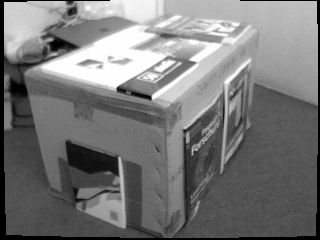
\includegraphics[width=.9\linewidth]{images/lab5-image1.png}
  \caption{Prvi pogled}
  \label{fig:lab5-image1}
\end{minipage}%
\begin{minipage}{.5\textwidth}
  \centering
  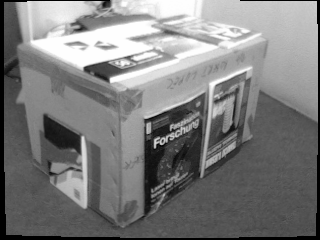
\includegraphics[width=.9\linewidth]{images/lab5-image2.png}
  \caption{Drugi pogled}
  \label{fig:lab5-image2}
\end{minipage}
\end{figure}

\newpage
\subsubsection{Prikaz point cloud-a}

\begin{figure}[h]
\centering
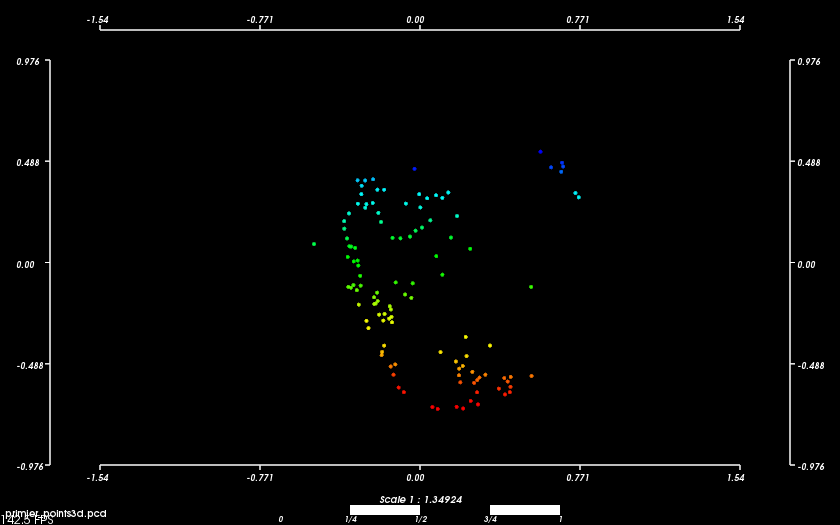
\includegraphics[scale=0.40]{images/lab5-pcd-01.png}
\caption{Point cloud prvi pogled}
\label{fig:lab5-pcd-01.png}
\end{figure}

\begin{figure}[h]
\centering
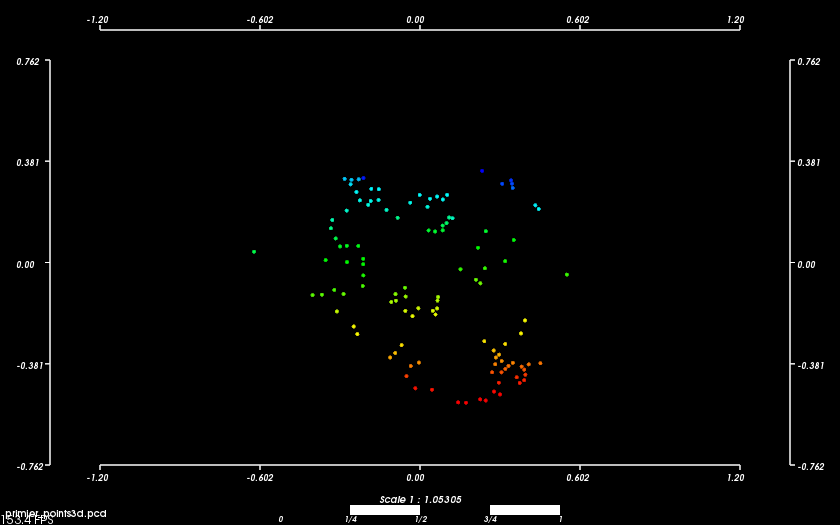
\includegraphics[scale=0.40]{images/lab5-pcd-02.png}
\caption{Point cloud drugi pogled}
\label{fig:lab5-pcd-02.png}
\end{figure}

\newpage
\subsection{Zaključak}
Cilj ove vježbe je bilo upoznati se rekonstrukcijom 3D prostora pomoću
dvije slike snimljene kalibriranom kamerom i poznatom projekcijskom
matricom. Nad slikama se SIFT-om određuju značajke te se pomoću deskritora
sparivaju s značajkama druge slike. Na temelju tih parova značajki
estimira se fundametalna matrica koja sadrži informacijju o epipolarnoj
geometriji kamera. Estimacija fundamentalne matrice se izvršava RANSAC
metodom kojom se ujedno i eliminiraju pogrešno sparene značajke. Na
temelju fundamentalne matrice i projekcijske matrice kamere određuje se
esencijalna matrica, koja sadrži informaciju o međusobnom položaju
kamera koja je neophodna za triangulaciju, odnosno izračunavanje
pozicija 3D točke u prostoru.
Za prikaz point cloud-a smo korstili pcl-viewer koji dolazi s pcl
bibliotekom i pruža prikaz točaka u prostoru te se mogu vidjeti
dobri rezultati programa.
